\section{Hypothesentests}
Basierend auf n unabhängig und identisch Verteilte (i.i.d) Zufallsvariablen $ X_{1}, ..., X_{n} $(Messungen) soll eine Entscheidung getroffen werden, ob eine Hypothese für einen unbekannten Erwartungswert $ \mu $ gültig ist or nicht.
\subsection{Def}
$\alpha $ = Signifikanzniveau/ Fehlerwahrscheinlichkeit 
TG = Prüfgröße; 
\subsection{Null- und Gegenhypothese}
\textbf{Modell:} Verteilung der Grundgesamtheit or Testgröße \textbf{TG} ( häufig $\overline{x}$ ) ist bekannt bis auf einen Parameter, z.B. $ \mu $, für den eine Hypothese aufgestellt wird.
$ TG \sim  N_{\mu, \sigma^2}$; 
\textbf{Nullhypothese: $ H_{0}$:} Angezweifelte Aussage, der widersprochen werden kann, wenn die Stichprobe einen Gegenbeweis liefert. $ H_{0}: \mu = \mu_{0}$; 
\textbf{Gegenhypothese $ H_{1} $:} Gegenteil von $ H_{0} $ z.B. $ H_{1} \neq \mu_{0} $;
\subsection{Ablehnungsbereich, Fehler 1. \& 2.}
Treffen der Testentscheidung, basierend auf einer konkreten Stichprobe 
$ \{x_{1}, ..., x_{n} \} $; Berechnung der Realisation $ tg = TG(x_{1},..., _x{n}) $ der Prüfgröße TG; 
\textbf{Ablehnungsbereich / Kritischer Bereich C}: Werte der Testgröße, die für H1, sprechen \& bei Gültigkeit von $ H_{0} $ mit Wahrscheinlichkeit $ \le \alpha $ ( meist 0.1, 0.05, or 0.01) auftreten.\textbf{Fehler 1. Art:}$ \alpha $ ist die Wahrscheinlichkeit, dass $ H_{0} $ verworfen wird, obwohl sie richtig ist.
\textbf{Annahmebereich:} Komplement $ \overline{C} $ des Ablehnungsbereichs. $ H_{0} $ kann nicht abgeleht werden, falls $ tg \in \overline{C} (P(tg \in \overline{C}) \ge 1 - \alpha) $.\textbf{Fehler 2. Art:} Die Wahrscheinlichkeit, dass $ H_{0} $ nicht abgelehnt wird, obwohl sie falsch ist.
  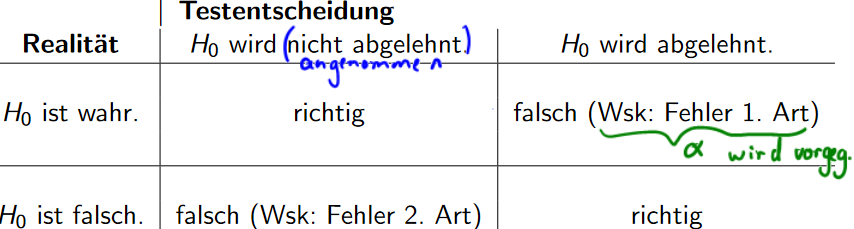
\includegraphics[scale=0.25]{./pic/Testzenarien.png}